\section{From polygon nests to triangle chords}\label{sec:chords}

The planar nesting estimate is now proved. We finish by using positive
flux identities to normalize the macroscopic triangle chords and calculate
their total marked mass. We first record a separate consequence of the
positive estimates: the weight $x$ is the critical step fugacity.

\subsection{An independent criticality consequence}

Let $c_n$ be the number of ordinary centre-to-centre self-avoiding walks
of $n$ edges from a fixed centre. We show that the series
$\sum_n c_n z^n$ has radius of convergence $x$. The decomposition is the
decreasing-span unfolding method associated with Hammersley and
Welsh~\cite{HammersleyWelsh1962}, in the present port convention.

Along the normal to a horizontal row, centre heights lie on a uniform
discrete mesh, and no dual bond is horizontal. Split a walk at its global
minimum height and reverse the first part. Each of the two resulting
walks is nonnegative relative to its starting height. In either part,
take the segment ending at the last vertex of maximum displacement from
its start, and repeat on the remainder with the sign reversed. Every
segment has positive span and has its two ends at its two extreme
heights. The spans strictly decrease after the first comparison, which
may be an equality. Their sum is $O(n)$, since the total variation of
height along an $n$-edge walk is $O(n)$. There are consequently
$O(\sqrt n)$ segments.

For a prescribed start, sign, and span, the total weight of such a
segment is bounded by an absolute constant. To see this, add boundary
legs at its two extremes to make it a crossing between parallel
horizontal triangle-side lines. If the outward bond at an extreme is
vertical, use its midpoint port. Otherwise first use a fixed slanted
outward bond to reach a new triangle with a vertical outward bond.
The additional centre lies strictly beyond the old extreme, so it is
unvisited. The two boundaries and the source port are determined by
the start, sign, and span up to finitely many lattice types, and deleting
the added legs has bounded multiplicity and bounded weight cost.
Exhausting the strip by finite convex parallelograms, the positive real
flux of Section~\ref{sec:cylinder} bounds the total crossing mass by an
absolute constant. The conversion between $x$ per edge and $x$ per
visited centre costs one further constant for each segment.

At a fixed starting centre, the minimum centre has only $O(n^2)$
possible positions. There are at most $n^{O(\sqrt n)}$ possible span
lists, and the product of the crossing bounds costs
$C^{O(\sqrt n)}$. Dropping endpoint and total-length constraints within
the segment sums therefore gives
\[
 c_nx^n\le \exp\bigl(O(\sqrt n\log(n+2))\bigr).
\]
The radius of convergence is at least $x$.

For the opposite inequality, half-plane saturation and the definition
of $D_N$ give the positive omitted mass
\[
 D_N=2\cos(3l)\left(
       \sum_{g\ge N}K_\infty(g)
       +\sum_{g=1}^{N-1}\bigl(K_\infty(g)-K_N(g)\bigr)\right)
       \asymp N^{-1/4}.
\]
Each omitted arc uses at least $a_{\rm len}N$ centres for an absolute
$a_{\rm len}>0$.
An arc in the first sum has endpoints separated by at least $N$; one
in the second meets a nonzero horizontal translate and hence has two
vertices separated by at least $N$. Deleting the port legs maps these
arcs to centre walks with bounded multiplicity, so for large $N$,
\[
 D_N\le C\sum_{n\ge a_{\rm len}N/2}c_nx^n.
\]
If the counting series had radius larger than $x$, choosing a fugacity
strictly between them would make this tail exponentially small in $N$.
This contradicts the polynomial lower bound. Thus the
radius is exactly $x$, at either centre type by lattice symmetry.
The denominator proof that follows uses the positive deficit and depth
estimates directly.

\subsection{The macroscopic chord denominator}

Put $\chi=\cos(3l)>0$ and write
\[
 B_\infty=2\sum_{g>0}K_\infty(g)=\chi^{-1}
\]
for the total half-plane arch mass from one boundary port, including both
endpoint directions. We will compare this saturated mass with the arches
that fit in a strip or a triangle.

\paragraph{Strip crossings.}
Let $B_d$ be the same-side arch mass in the infinite strip of width $d$
rows from a fixed source port, and let $S(d)$ be its mass of crossings to
the opposite parallel boundary. In a finite convex parallelogram
$\Pi$ exhausting this strip, the same-side exits have cosine $\chi$,
the opposite-side exits have cosine one, and the real flux through the
two end sides is nonnegative. With the analogous finite masses this is
\[
 1=\chi B_\Pi+S_\Pi+E_\Pi^{\rm end},
 \qquad E_\Pi^{\rm end}\ge0.
\]
Monotone exhaustion of the two indicated path classes gives the strip
missing-mass inequality
\begin{equation}\label{eq:strip-missing-mass}
 S(d)\le 1-\chi B_d=\chi(B_\infty-B_d).
\end{equation}

The strip contains every quotient-self-avoiding arc of positive span
$g<N$ and depth less than $d-C_{\rm lat}$, and also its reflected
negative-span copy. Therefore, for any $N<d-C_{\rm lat}$,
\begin{equation}\label{eq:strip-quotient-bound}
 \begin{split}
 S(d)
 &\le D_N+
 2\chi\sum_{g=1}^{N-1}
       \sum_{\substack{\gamma\in\mathscr A_N(g)\\
                        \operatorname{dep}(\gamma)\ge d-C_{\rm lat}}}
             w(\gamma).
 \end{split}
\end{equation}
Here we used $1-2\chi\sum_{g<N}K_N(g)=D_N$. Choose
$N=\lfloor\rho d\rfloor$ with a fixed small $\rho>0$ so that
$(d-C_{\rm lat})/N-C_*>1$ for all large $d$. The depth sum is then
$O(N^{-1/4})$ by \eqref{eq:arc-depth-moments}, already with $k=1$.
Proposition~\ref{prop:cylinder} bounds $D_N$ by the same order.
Increasing the constant for bounded $d$ proves
\begin{equation}\label{eq:strip-crossing-bound}
 S(d)\le C d^{-1/4}.
\end{equation}
The bound holds for each of the finitely many source types and their
lattice rotations.

\paragraph{Triangle flux and a parallel cut.}
For a source port $a$ on one side of an equilateral lattice triangle
$\Delta$, let $B_\Delta(a)$ be the unsigned mass of paths returning to
that side, and let $E_\Delta(a)$ be the unsigned mass of paths exiting
on either of the other sides. A same-side chord has total turn
$\pm\pi$, while a chord to another side has total turn $\pm\pi/3$.
The finite real flux identity is therefore
\begin{equation}\label{eq:triangle-flux}
 \chi B_\Delta(a)+\cos(l)E_\Delta(a)=1,\qquad
 \cos(l)E_\Delta(a)=\chi\bigl(B_\infty-B_\Delta(a)\bigr).
\end{equation}
This identifies the other-side exits with the half-plane arch mass lost
by restricting the paths to the triangle.

Clip $\Delta$ by a parallel lattice cut at inward depth $d$ rows from
the source side, and retain the component $\Delta_{\le d}$ containing
that side. Let $\mathcal L_d(a)$ be the paths from $a$ to the original
boundary that use a removed triangle, and let $\mathcal Q_d(a)$ be the
paths in $\Delta_{\le d}$ from $a$ to the new cut. Subtract the real
flux identities before and after clipping. Every path that remains in
the clipped domain and exits on an original side cancels. The new cut
is parallel to the source side, so its exits have total turn zero.
The exact remaining identity and its consequence are
\begin{equation}\label{eq:triangle-cut-flux}
 \begin{gathered}
 \sum_{\gamma\in\mathcal L_d(a)}w(\gamma)\cos(cW(\gamma))
       =\sum_{\gamma\in\mathcal Q_d(a)}w(\gamma)\le S(d),\\
 \sum_{\gamma\in\mathcal L_d(a)}w(\gamma)
       \le \chi^{-1}S(d)\le C d^{-1/4}.
 \end{gathered}
\end{equation}
The last inequality uses $\cos(cW)\ge\chi$ on every convex triangle
chord. In particular it bounds all exits whose paths reach beyond the
parallel cut.

\paragraph{The half-plane diameter tail.}
Let $\mathcal H(r)$ be the total mass of half-plane arches from a fixed
port, in both directions, with diameter at least $r$. For large $r$,
inscribe an equilateral lattice triangle of side $\lfloor r/2\rfloor$
in the half-plane with its base on the boundary. From any port $a$ in
the central third of the base, every such arch is missing from the
triangle, whose diameter is less than $r$. Equation
\eqref{eq:triangle-flux} gives
\[
 \chi\mathcal H(r)\le \cos(l)E_\Delta(a).
\]
Sum over these order-$r$ base ports and reverse the paths on the right.
From each source on a slanted side, the reversed paths reach a central
base port, whose distance from that side is at least a fixed positive
multiple of $r$. They therefore reach beyond a parallel cut of depth
$c_2r$ rows, with an absolute $c_2>0$ and harmless integer rounding.
Equation \eqref{eq:triangle-cut-flux}, summed over the $O(r)$ slanted
ports, yields
\[
 c_3r\,\mathcal H(r)\le C r S(c_2r)\le C r^{3/4}.
\]
Translation invariance makes $\mathcal H(r)$ the same for every central
base source. We have proved
\begin{equation}\label{eq:halfplane-diameter-tail}
 \mathcal H(r)\le C r^{-1/4}.
\end{equation}

\paragraph{Integrating both endpoints.}
For a fixed $\delta>0$, let $\mathcal C_R(\delta)$ be the ordered
boundary-to-boundary paths in $\Delta_R$ of diameter at least $\delta R$,
and put $Z_R(\delta)=\sum_{\gamma\in\mathcal C_R(\delta)}w(\gamma)$.
We claim
\begin{equation}\label{eq:chord-cutoff-denominator}
 Z_R(\delta)\asymp_\delta R^{3/4}
 \qquad\text{for every fixed }0<\delta\le1/50.
\end{equation}
The comparison constants may depend on the fixed cutoff $\delta$.

For the upper bound, same-side paths from each port have mass at most
$\mathcal H(\delta R)=O_\delta(R^{-1/4})$. For paths to another side,
let $r$ be the source port's distance along its side to the nearer
corner. Every half-plane arch missing from the triangle has reached a
slanted side, at distance at least $c_4r-C_{\rm lat}$ from the source.
It thus has diameter of that order. By
\eqref{eq:triangle-flux} and \eqref{eq:halfplane-diameter-tail}, all
other-side exits from that port have mass at most $Cr^{-1/4}$ when
$r$ exceeds a fixed constant. The bounded number of ports closer to
corners have bounded mass by finite flux. Summing over the $O(R)$
sources gives
\[
 Z_R(\delta)\le C_\delta R^{3/4}
             +C\sum_{r=1}^{R}r^{-1/4}
       \le C_\delta R^{3/4}.
\]

For the lower bound take a source in the central third of the base and
put $N=3R$. Every triangle base-to-base arch projects self-avoidingly to
this quotient: the triangle has horizontal width $R<N$, and its endpoint
span has absolute value less than $N$. Thus
\[
 B_{\Delta_R}(a)\le2\sum_{g=1}^{3R-1}K_{3R}(g),\qquad
 \cos(l)E_{\Delta_R}(a)\ge D_{3R}.
\]
The source has distance at least $\sqrt3R/6$ from either slanted line,
so every other-side exit has diameter greater than $R/50$. Summing over
the order-$R$ central base ports proves
$Z_R(\delta)\ge C^{-1} R D_{3R}\ge C^{-1}R^{3/4}$ for the stated range of
$\delta$. This proves \eqref{eq:chord-cutoff-denominator}; the
denominator in Theorem~\ref{thm:triangle} is $Z_R(1/100)$.

\subsection{The edge-slit identity}

To compute the length numerator, fix an interior side midpoint $e$ of
the tiling. Cutting the honeycomb edge at $e$ creates two slit ports,
one facing each adjacent triangle. For this subsection paths may have
any diameter. Let
\[
 T_e=\sum_{\substack{\gamma\text{ boundary-to-boundary}\\e\in\gamma}}
 x^{m(\gamma)}\cos(cW(\gamma)),\qquad c=3/8,
\]
where both endpoint orders are counted and $W$ includes the first and
last turns. Define $Z_e$ to be the partition function of disjoint simple
polygons in $\Delta_R$ avoiding and enclosing $e$, with weight
$2x^{|P|}$ per polygon. Define $L_e$ by additionally marking one
disjoint polygon through $e$: this polygon has weight $x^{|P|}$,
while every other polygon still has weight $2x^{|P|}$ and encloses $e$.

\begin{figure}[t]
\centering
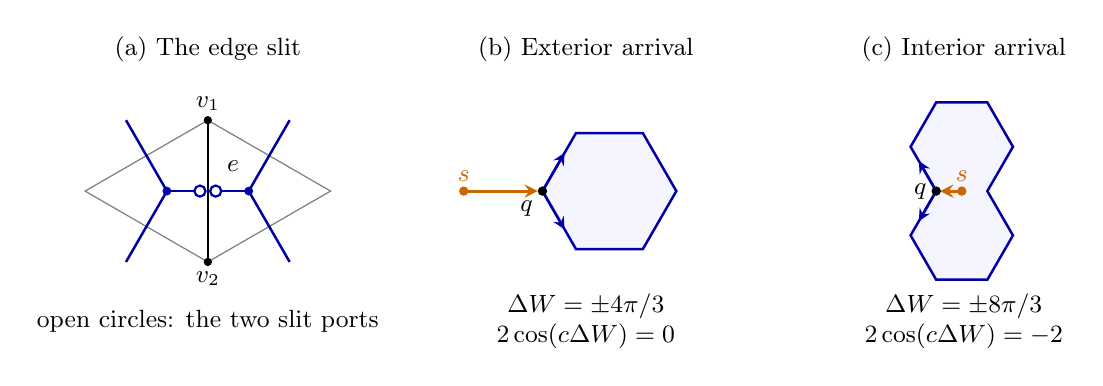
\begin{tikzpicture}[x=1cm,y=1cm,>=stealth,font=\small,
  primal/.style={draw=black!50,line width=.45pt},
  dual/.style={draw=blue!65!black,line width=.9pt},
  arrival/.style={draw=orange!80!black,line width=1.1pt,->}]
\begin{scope}
  \node at (0,1.8) {(a) The edge slit};
  \draw[primal] (0,.9)--(-1.55885,0)--(0,-.9)
                (0,.9)--(1.55885,0)--(0,-.9);
  \draw[black,line width=.7pt] (0,.9)--(0,-.9);
  \draw[dual] (-1.03923,.9)--(-.519615,0)--(-1.03923,-.9)
              (1.03923,.9)--(.519615,0)--(1.03923,-.9);
  \draw[dual] (-.519615,0)--(-.10,0)
              (.10,0)--(.519615,0);
  \fill[blue!65!black] (-.519615,0) circle(1.6pt);
  \fill[blue!65!black] (.519615,0) circle(1.6pt);
  \draw[blue!65!black,fill=white,line width=.8pt]
        (-.10,0) circle(2pt) (.10,0) circle(2pt);
  \fill (0,.9) circle(1.5pt) node[above] {$v_1$};
  \fill (0,-.9) circle(1.5pt) node[below] {$v_2$};
  \node[above right] at (.12,.13) {$e$};
  \node[align=center] at (0,-1.65)
    {open circles: the two slit ports};
\end{scope}
\begin{scope}[xshift=4.8cm]
  \node at (0,1.8) {(b) Exterior arrival};
  \path[fill=blue!4] (-.55,0)--(-.125,.736122)--(.725,.736122)
      --(1.15,0)--(.725,-.736122)--(-.125,-.736122)--cycle;
  \draw[dual] (-.55,0)--(-.125,.736122)--(.725,.736122)
      --(1.15,0)--(.725,-.736122)--(-.125,-.736122)--cycle;
  \draw[dual,->] (-.55,0)--(-.27,.484974);
  \draw[dual,->] (-.55,0)--(-.27,-.484974);
  \draw[arrival] (-1.55,0)--(-.61,0);
  \fill[orange!80!black] (-1.55,0) circle(1.7pt)
      node[above] {$s$};
  \fill (-.55,0) circle(1.7pt) node[below left] {$q$};
  \node[align=center] at (0,-1.65)
    {$\Delta W=\pm4\pi/3$\\$2\cos(c\Delta W)=0$};
\end{scope}
\begin{scope}[xshift=9.6cm]
  \node at (0,1.8) {(c) Interior arrival};
  \path[fill=blue!4] (-.35,0)--(-.675,.562917)--(-.35,1.125834)
      --(.30,1.125834)--(.625,.562917)--(.30,0)
      --(.625,-.562917)--(.30,-1.125834)--(-.35,-1.125834)
      --(-.675,-.562917)--cycle;
  \draw[dual] (-.35,0)--(-.675,.562917)--(-.35,1.125834)
      --(.30,1.125834)--(.625,.562917)--(.30,0)
      --(.625,-.562917)--(.30,-1.125834)--(-.35,-1.125834)
      --(-.675,-.562917)--cycle;
  \draw[dual,->] (-.35,0)--(-.57,.381051);
  \draw[dual,->] (-.35,0)--(-.57,-.381051);
  \draw[arrival] (-.025,0)--(-.30,0);
  \fill[orange!80!black] (-.025,0) circle(1.7pt)
      node[above] {$s$};
  \fill (-.35,0) circle(1.7pt) node[left] {$q$};
  \node[align=center] at (0,-1.65)
    {$\Delta W=\pm8\pi/3$\\$2\cos(c\Delta W)=-2$};
\end{scope}
\end{tikzpicture}
\caption{The slit and the two first-repeat cancellations, with $c=3/8$.
In (a), black and grey segments are primal tiling sides and blue segments
are honeycomb bonds. The bond crossing the side $v_1v_2$ is cut at its
midpoint $e$; the two slit ports are separated slightly for visibility.
Panels (b) and (c) are schematic representatives. The orange leg is
the first prefix arrival at $q$ from the slit source $s$. The path then
traverses the blue cycle and returns to $q$, its first repeated dual
vertex. The two arrows leaving $q$ indicate the two cycle
orientations. Their additional rotations are $\pm4\pi/3$ when $s$ is
outside the cycle and $\pm8\pi/3$ when $s$ is inside. In (c), the arrival
leg occupies the reflex interior sector at $q$.}
\label{fig:slit}
\end{figure}


\begin{lemma}[Slit flux]\label{lem:slit}
For every interior contact $e$,
\[
 T_e=2Z_e+\sqrt2L_e.
\]
Consequently $T_e$ is comparable, with absolute positive constants,
both to the unsigned chord mass through $e$ and to the sum of the
enclosing polygon partition functions at the two endpoints of the
primal tiling side containing $e$.
\end{lemma}

\begin{proof}
First run the finite boundary exploration of Section~\ref{sec:cylinder}
from an outer port, allowing it to stop on the slit. The cancellation
at a previously visited triangle is unchanged. Subtract this flux
identity from the identity without the slit, and sum over all outer
sources. The unchanged outer exits cancel, leaving the chords through
$e$ and the stopped outer-to-slit paths. Reversal changes the sign of
$W$ and preserves its cosine, so
\begin{equation}\label{eq:slit-comparison}
 \begin{split}
 T_e&=\sum_{\gamma\text{ outer-to-slit}}
                x^{m(\gamma)}\cos(cW(\gamma))\\
 &=\sum_{\gamma\text{ slit-to-outer}}
                x^{m(\gamma)}\cos(cW(\gamma)).
 \end{split}
\end{equation}
The last sum uses both slit sources. All explorations are finite, so
this subtraction requires no limiting argument.

Now fix one slit source $s$ and run the same exploration in the
presence of a polygon configuration counted by $Z_e$. Its initial
mass, summed over those configurations, is $Z_e$. At a fresh
unoccupied triangle, extend through either of the other sides. The
two weighted phases sum to one. Stop a branch at an exit, a first
repeated triangle, or the first hit on a gas polygon.

The two first-repeat cases are illustrated in Figure~\ref{fig:slit}.
At a repeated triangle $q$, the two orientations of the resulting
path-cycle have the same positive weight. If the source lies outside
the cycle, their extra rotations after the first prefix arrival at
$q$ are $\pm4\pi/3$, and their phases sum to zero, as in the boundary
exploration. If the source is inside, the prefix arrives from the
interior. The unused third leg is then in the reflex interior sector
of the cycle. For counterclockwise traversal the cycle's turn at $q$
is $-\pi/3$, while the prefix takes turn $+\pi/3$. The two rotations
added after the first arrival are therefore $\pm8\pi/3$, and their
phases sum to
\[
 2\cos(8\pi c/3)=-2.
\]
These terminal terms cancel the first-hit terms for which that cycle
is an independent gas polygon of weight $2x^{|P|}$. The correspondence
keeps all other polygons fixed. Indeed a gas polygon encloses $s$,
so its first hit is from its interior; the prefix before that hit is
disjoint from the polygon and from all remaining gas polygons.
Removing the hit polygon and traversing it in either orientation
gives exactly the two first-repeat branches. Conversely, a first
repeated cycle enclosing $s$ is disjoint from the earlier prefix apart
from its attachment at $q$, and is disjoint from the remaining gas
polygons, so it can be installed as that gas polygon.
The weights agree because the extensions visit each cycle triangle once.

An outer exit cannot coexist with a gas polygon enclosing the slit
source. Let $O_s$ be the real mass of these outer exits, with no gas
polygon present. The remaining slit exits return from the opposite
side of $e$ and close a polygon through $e$. Their total turn is
$\pm2\pi$. With the initial side prescribed, each such marked polygon
is represented once and has real factor
$\cos(2\pi c)=-1/\sqrt2$. Taking real parts in the one-source
conservation identity gives
\[
 Z_e=O_s-\frac{L_e}{\sqrt2},
 \qquad O_s=Z_e+\frac{L_e}{\sqrt2}.
\]
Adding the two slit sources and using \eqref{eq:slit-comparison}
proves the identity.

Let $v_1,v_2$ be the primal vertices at the ends of the side containing
$e$, and let $\mathcal Z^{\Delta_R}_{v_i}$ be their enclosing polygon
partition functions restricted to $\Delta_R$. A dual polygon avoiding
$e$ cannot cross the open primal side, so if it encloses either $v_i$,
it encloses both and also $e$. A polygon through $e$ encloses exactly
one of these vertices, and at most one polygon in a disjoint nest can
pass through $e$. Decomposing by these alternatives gives
\[
 \mathcal Z^{\Delta_R}_{v_1}+\mathcal Z^{\Delta_R}_{v_2}=2Z_e+2L_e,
\]
which is comparable to $2Z_e+\sqrt2L_e$ with absolute positive
constants. Finally, convex boundary flux gives
\[
 \cos(3\pi/8)\sum_{\gamma\ni e}x^{m(\gamma)}
 \le T_e\le\sum_{\gamma\ni e}x^{m(\gamma)}.
\]
This proves the other comparison.
\end{proof}

\subsection{The length numerator and the mean}

Let $A_e$ be the unsigned mass of all ordered boundary chords through
$e$. The planar nesting estimate and Lemma~\ref{lem:slit} give
\[
 A_e\le R^{1/12+o(1)}
\]
uniformly over contacts in the triangle. If $e$ lies in the concentric
triangle of side $R/3$, both adjacent primal vertices have distance
comparable to $R$ from the boundary. For fixed positive
$a_{\rm in},a_{\rm out}$, domain inclusion gives
\[
 \mathcal Z_{v_i}(a_{\rm in}R)
 \le\mathcal Z_{v_i}^{\Delta_R}
 \le\mathcal Z_{v_i}(a_{\rm out}R),\qquad i=1,2.
\]
Monotonicity therefore gives
$A_e=R^{1/12+o(1)}$ uniformly throughout that central region.
The distance from the concentric triangle of side $R/3$ to the
boundary of $\Delta_R$ is $\sqrt3R/9$. Thus every chord through a
central contact has diameter at least $\sqrt3R/9$, and in particular
belongs to $\mathcal C_R(\delta)$ for every fixed $0<\delta\le1/50$.

There are order $R^2$ central contacts and at most order $R^2$
contacts altogether. A path visiting $m$ centres crosses exactly
$m-1$ interior contacts. Define
$M_R(\delta)=\sum_{\gamma\in\mathcal C_R(\delta)}m(\gamma)w(\gamma)$.
For each fixed $0<\delta\le1/50$,
\begin{equation}\label{eq:chord-cutoff-numerator}
 \begin{split}
 M_R(\delta)
 &=Z_R(\delta)+
   \sum_e\sum_{\substack{\gamma\in\mathcal C_R(\delta)\\e\in\gamma}}
        w(\gamma)\\
 &=R^{25/12+o(1)}.
 \end{split}
\end{equation}
The lower bound uses the central contacts, for which all chords are
admissible. The upper bound allows all chords at every contact.
Dividing \eqref{eq:chord-cutoff-numerator} at $\delta=1/100$ by
\eqref{eq:chord-cutoff-denominator} proves the port mean assertion in
Theorem~\ref{thm:triangle}.

We finish with an explicit comparison for ordinary centre walks.
Let $\mathcal W_R(\delta)$ be the ordered centre-to-centre walks
contained in $\Delta_R$, with both endpoints on its inner boundary
layer and diameter at least $\delta R$. If $n(\omega)$ is their number
of edges, put
\[
 \begin{gathered}
 Z_R^\circ(\delta)=\sum_{\omega\in\mathcal W_R(\delta)}x^{n(\omega)},\\
 M_R^\circ(\delta)=
       \sum_{\omega\in\mathcal W_R(\delta)}(n(\omega)+1)x^{n(\omega)}.
 \end{gathered}
\]
Every such walk has at least one extension by boundary half-edges to
two ports, and at most $Q=9$ extensions, since each endpoint triangle
has at most three boundary sides. Deleting the two half-edges recovers
the walk. An extension has exactly $m=n+1$ visited centres and weight
$x^{n+1}=x\,x^n$. Moreover, for an absolute $b$,
\[
 \diam(\omega)\le\diam(\text{port extension})
                 \le\diam(\omega)+b.
\]
Take the two fixed cutoffs $\delta_0=1/100$ and $2\delta_0=1/50$.
For all large $R$, deleting the half-edges from a chord of diameter
at least $2\delta_0R$ leaves a centre walk of diameter at least
$\delta_0R$; every extension of a centre walk at cutoff $\delta_0$
is itself a chord at that cutoff. The weight and multiplicity bounds
give the two squeezes
\begin{equation}\label{eq:centre-cutoff-squeeze}
 \begin{gathered}
 \frac{Z_R(2\delta_0)}{xQ}\le Z_R^\circ(\delta_0)
       \le\frac{Z_R(\delta_0)}x,\\
 \frac{M_R(2\delta_0)}{xQ}\le M_R^\circ(\delta_0)
       \le\frac{M_R(\delta_0)}x.
 \end{gathered}
\end{equation}
Both cutoffs lie in the fixed range already proved. Hence
$Z_R^\circ(\delta_0)\asymp R^{3/4}$ and
$M_R^\circ(\delta_0)=R^{25/12+o(1)}$. Their ratio is the mean of
$n+1$, so the mean edge length is
$M_R^\circ(\delta_0)/Z_R^\circ(\delta_0)-1=R^{4/3+o(1)}$.
This proves the centre-to-centre assertion.
